\section{Nombre: Cimatl}  \label{per:cimatl}
\subsection{Descripción:} 
Mujer de edad media. Cimatl es una mujer bella, de piel morena y cabello largo. Lleva el pelo recogido en una especie de chongo como el que usaban las mujeres nobles de la capital del imperio. Viste una especie de chal que le llega hasta la altura de los codos y un huipil cuyo largo es hasta los tobillos. Una un par de pulseras de jade, una en cada mano y un collar de oro labrado por Mixtecos por lo que tiene una gran cantidad de detalles en su labrado. Ademas de eso, utiliza un par de aretes labrados en la misma zona. Porta unas sandalias que cubren la mayor parte de sus pies.
\\
\par
Cimatl es una mujer ambiciosa que se siente atraída al poder. Su deseo por el poder es tal que no durara en hacer lo que sea necesario para mantenerse en el poder y gozar de la riqueza.        
\subsection{Status:}
\begin{itemize}
		\item Personaje no jugable.
	\end{itemize}
Es uno de los fantasmas del pasado de Malinalli.
\subsection{Imagen}
Ver figura \ref{fig:CimatlDiseno}
	\begin{figure}
					\centering
					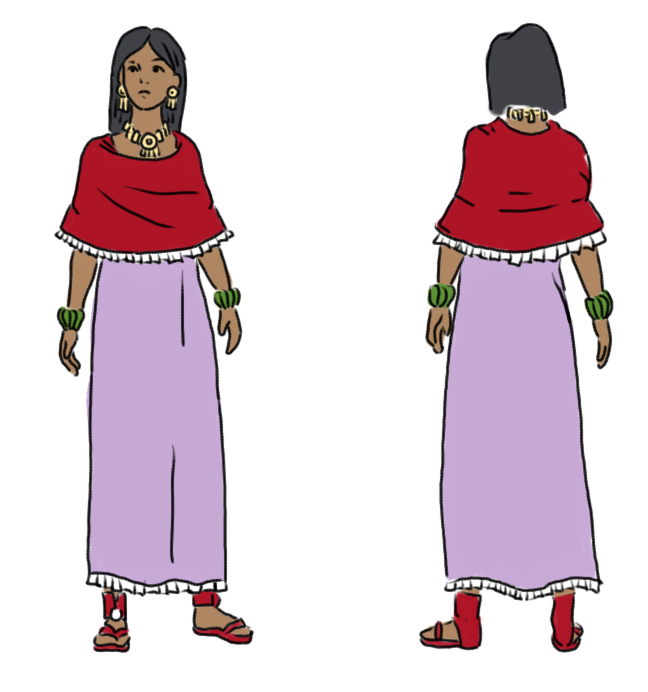
\includegraphics[height=0.3 \textheight]{Imagenes/Cimatl}
					\caption{Concepto de diseño de Cimatl.}
					\label{fig:CimatlDiseno}
	\end{figure}
\subsection{Concepto:}
\begin{itemize}
	\item \textbf{Historia antes del juego:}
	Hija de un importante comerciante. Durante su juventud Cimatl tuvo un sin numero de pretendientes que deseaban esposarla por su gran belleza; sin embargo, Cimatl no encontraba en ninguno de sus pretendientes alguno que le garantizara una posición social de mayor rango de la que ya gozaba. Gracias a la amistad de su padre con uno de los consejeros del nuevo cacique, los padres de Cimatl arreglaron el matrimonio de su hija con el cacique. La vida matrimonial solo logro decespcionar a Cimatl, ya que ella esperaba que su esposo fuera un hombre ambicioso y en su lugar encontro un hombre preocupado por su pueblo y no en el poder. Por lo que Cimatl empieza a temer por la seguridad de su patrimonio al temer que su esposo perdiera el poder por su antitud amable.
	\\
	\par
	Después de varios años de matrimonio, Cimatl queda embarazada; a lo que ella empezaría a depositar sus esperanzas de conseguir más poder al dar a luz a un varón. Pero sus planes se ven truncados con el nacimiento de una niña. A los años que siguieron de su matrimonio, Cimatl comenzó a proponerle a su esposo la idea de conseguirle a futuro un arreglo matrimonial a Malinanlli con algún importante señor de la capital del imperio a lo que Tenépal se niega, ganandose la furia de su esposa.
	\\
	\par
	Su oportunidad para hacerse de más poder llega cuando descubre la conspiración que su esposo estaba orquestando contra el imperio. Cimatl, temerosa de que su esposo fuera descubierto y ello significara la ruina de ella, decide entregarlo al tlatoani con la condición de que ella sería la esposa del siguiente cacique.
	\\
	\par
	A los pocos meses de la muerte de su espos, Cimatl contrae nupcias con el nuevo cacique de Oluta. De este matrimonio nacería un hijo varón, que se convertiría en la llave de más poder para Cimatl. Es entonces cuando Malinalli comienza a ser una amenaza para sus pretensiones políticas por lo que decide venderla como una esclava.  
	\item \textbf{Historia durante el juego:}
	Se conocerá a Cimatl a través de los recuerdos de Malinalli ya que no tiene participación en la historia que transcurre dentro del Mictlán.
	\item \textbf{Relaciones:}
	\begin{itemize}
		\item \textbf{Tenépal:} Considerado como un hombre débil y de poca visión por su esposa. Ella lo aborrecía al ser un obstáculo a sus pretensiones de poder (ver aparatado \ref{per:tenepal}). 
		\item \textbf{Malinalli:} vista como el mayor fracaso de Cimatl, ya que por su condición de mujer no resultaba provechosa para mantener la posición política de su madre ni su riqueza. Con el nacimiento de su hermano, Malinalli pasa a ser una amenaza para Cimatl por lo que debe de ser erradicada (ver aparatado \ref{per:malinalli}).
		\item \textbf{Huenupan:} Segundo esposo de Cimatl. No guarda amor por el pero lo considera útil (ver aparatado \ref{per:huenupan}).
	\end{itemize}                     
\end{itemize}

\subsection{Encuentro:}
Aparece por primera vez en la cinemática 25 (ver aparatado \ref{Cin:Cinematica25}).
\subsection{Habilidades:}
Su principal habilidad es la de planear y conspirar para obtener lo que desea.
\subsection{Armas:}
No posee armas ni esta amaestrada en la batalla.
\subsection{Ítems:}
Sin ítems.
\subsection{Bloques de animación}
\begin{itemize}
	\item Animación caminar.
	\item Animación normal.
	\item Animación sentada.
	\item Animación sentada con bebé en brazos.
\end{itemize}